\documentclass[12pt]{article}
\usepackage[utf8]{inputenc}
\usepackage[T1]{fontenc}
\usepackage{lmodern}
\usepackage{graphicx}
\usepackage{subcaption}
\usepackage[svgnames]{xcolor}
\usepackage[a4paper,bindingoffset=0.2in,%
            left=0.5in,right=0.5in,top=0.5in,bottom=1in,%
            footskip=.25in]{geometry}
\pagenumbering{gobble}
\usepackage[colorlinks=true, linkcolor=Black, urlcolor=Blue]{hyperref}

\begin{document}
\title{Sprawozdania z zajęć z prototypowania}
\author{Sebastian Michoń 136770, Mateusz Wankowski 136823,\\ Piotr Król XXXXXX, Maciej Leszczyk 136759}
\date{\vspace{-3ex}}
\maketitle

\section{Idee, koncepcje, motywacje}
Ideą naszego prototypu było stworzenie aplikacji \underline{wspomagania systemu kolejkowego}, podobnej do politechnicznego \underline{Zintegrowanego Centrum Obsługi}. Uznaliśmy, że aplikacja politechniczna jest wysoce niedoskonała, skłoniło nas to do pokazania światu nowej, po wielokroć wspanialszej wersji tego systemu, z liczbą opcji, o których paniom z dziekanatu się nie śniło. Nasz aplikacja powinna mieć charakter mobilny, co umożliwi korzystanie z niej poza politechniką.

\section{I etap prototypowania}
\subsection {Indywidualne pomysły}
\begin {enumerate}
	\item Pierwsza koncepcja indywidualna Piotra to możliwość stwierdzenia przy pobraniu biletu, o której dana osoba wchodzi do dziekanatu i czy zgadza się na przesuwanie jej w kolejce na wcześniejszy termin: uznaliśmy, że jeśli osoba ma termin wizyty o kilka godzin późniejszy niż termin pobrania biletu, może chcieć np. zjeść obiad w trakcie czasu oczekiwania - natomiast jeśli i tak czeka w poczekalni, może się zgodzić na przesuwanie jej na jak najwcześniejszy termin jeśli np. jakaś wizyta potrwa krócej niż oczekiwano.
	
	\item Mateusz zauważył, że jeśli ktoś woli czekać w kolejce, to zapewne nie ma niczego ciekawszego z jego perspektywy niż wchodzenie w interakcję z innymi ludźmi - a co za tym idzie, dobrze by było, gdyby nasza aplikacja była wyposażona w substytut messengera predestynowany dla ludzi partycypujących w naszym systemie kolejkowym. Funkcjonalność ta uwzględnia możliwość dołączenia do czatu grupowego dla wszystkich osób będących w kolejce, oraz wysyłania wiadomości prywatnych. Wiadomości prywatne można jednak wysyłać tylko do osób które zgodziły się na otrzymywanie wiadomości od innych użytkowników zaznaczając odpowiedniego checkboxa.
	
	\item Pomysł Macieja polegał na możliwości przeglądania osób znajdujących się razem z nami w kolejce. Po zalogowaniu się i dołączeniu do poczekalni widzimy swoje informacje personalne wraz ze zdjęciem, numerkiem w kolejce oraz szacowanym czasem oczekiwania. Oprócz tego interfejs wyposażony jest w guziki next i previous dzięki którym możemy dostrzec analogiczne informacje o innych uczestnikach z kolejki. Idea ta wydawała się dziwna i niepotrzebna, jednak połączyliśmy ją z poprzednim pomysłem i dzięki temu możemy wchodzić w konwersację prywatną z innymi użytkownika korzystając właśnie z tego interfejsu.	
	
	\item Michoń spostrzegł, że dobrze by było, gdyby osoba zalogowana do systemu miała możliwość obejrzenia swojej historii wizyt w dziekanacie - żeby przypomnieć sobie, z kim ostatnio prowadziła konwersację np. żeby później móc dostarczyć mailem zaległą informację, której nie była w stanie podać w trakcie wizyty.

\end {enumerate}

\subsection {Co wspólne, co różne}
Wspólną cechą wszystkich projektów były 2 funkcjonalności różne od głównej - możliwość zalogowania się do systemu albo anonimowego użytkowania aplikacji, a także szacowanie czasu pozostałego do wizyty. Różne indywidua wysnuwały jednakże różne wnioski z tych funkcjonalności - jedni opierali o nie funkcjonalność chatu, inni historię i zgodę na przesuwanie w kolejce. Poza tymi 2 kwestiami wszystko inne było różne.

\subsection{Co okazało się dobrym pomysłem, co nie}
\begin {enumerate}
	\item Chat okazał się niezgorszym pomysłem, uznaliśmy, że wielu jest ludzi pragnących w trakcie oczekiwania w kolejce prowadzić konwersację z innymi personami. 
	
	\item Możliwość stwierdzenia, czy osoba woli być przesuwana także jest opcją, która jest z naszej perspektywy bardzo zasadna - przy długim czasie oczekiwania czasem nie ma sensu siedzieć w kolejce, lepiej wyjść i zająć się czymś innym przed wizytą.
	
	\item Historia poprzednich wizyt okazała się przeciętnym pomysłem, niektórzy uważają, że jej jedynym zastosowaniem jest sprawdzenie, ile czasu swojego życia zmarnowało się w niezrównanym królestwie biurokracji zwanym dziekanatem, niemniej jednak może stanowić niemałą pomoc dla ludzi roztargnionych i nierozgarniętych, dlatego zdecydowaliśmy się ją uwzględnić w II etapie projektowania apikacji.
	
\end {enumerate}

\section {Wnioski z II etapu projektowania aplikacji}
\subsection {Które pomysły zostały zrealizowane, które nie?}

Wszystkie indywidualne pomysły zostały zaimplementowane w naszej aplikacji, jednak część z nich w inny sposób niż wyobrażał to sobie autor.

\subsection{Które pomysły okazały się trafione, które nie według osób spoza grupy?}
\begin{enumerate}
	\item Trafionym pomysłem okazał się chat - ludzie spoza grupy byli bardzo skorzy do korzystania z tej funkcjonalności aplikacji, może nawet bardziej niż z jej głównej funcjonalności
	\item Historia wzbudzała kontrowersje - jedni twierdzili, że jest absolutnie zbędna, inni, że może być bardzo pomocna w dostarczaniu zaległych informacji.
\end{enumerate}


\section {Aplikacja w akcji}
\clearpage

\begin{figure}[h!]
	\centering
	\begin{subfigure}[b]{1\linewidth}
		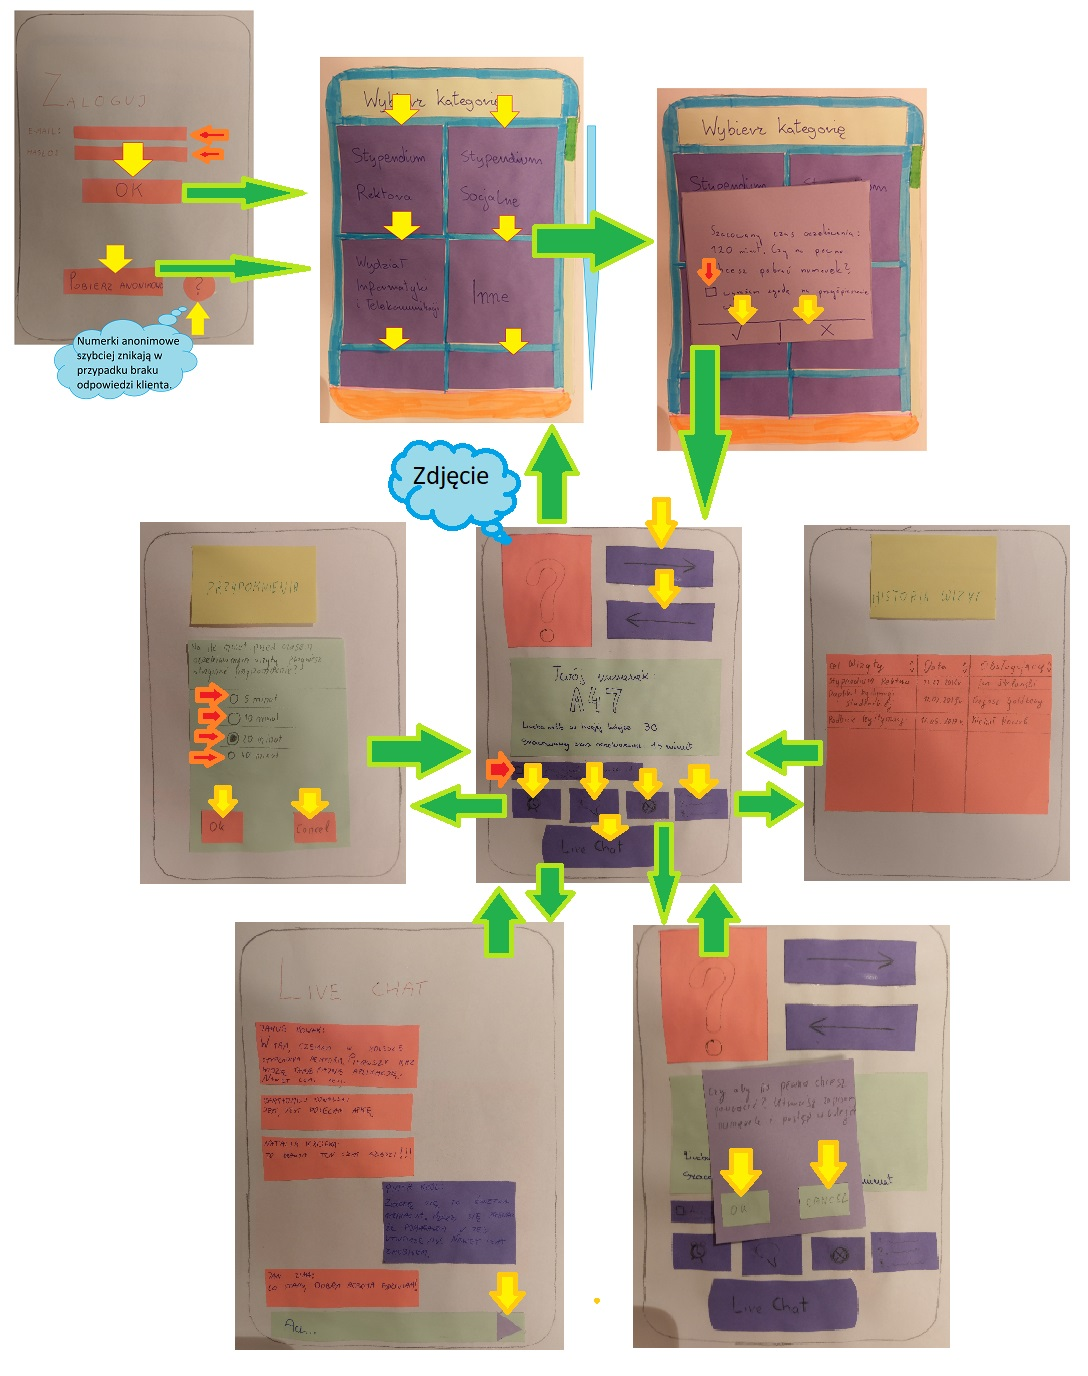
\includegraphics[width=\linewidth]{zdj/mozaika.jpg}
		\caption{Podpis}
	\end{subfigure}
	\label{fig:nuty}
	\caption{Nawigacja}
\end{figure}

\end{document}
